\chapter{Description and analysis of existing test framework} 
\label{Chapter3} 

In a project like the Serval project, confidence in its performance is crucial — particularly if it will be used in disaster recovery efforts.
To achieve this, both the development team and potential users of the network need to be confident in its performance in a wide range of scenarios. 
While a significant portion of this will need to be done through field testing, this is unfeasible to perform without software emulation.

The test frameworks for Serval-DNA and LBARD were developed to perform software testing by emulating the real Serval software and analysing its behaviour during tests.
In this chapter, the first research question "\firstRQ" will continue to be answered as was started in Chapter 2. 


\section{Aims of test frameworks}
The Serval-DNA test framework was built to test the functionality of the Serval mesh in its early days when nodes were purely communicating over WiFi. 
This emulator is able to emulate multiple aspects of the Serval DNA software, from validating the database integrity to simulating WiFi communication between Serval nodes. 
Later, once LBARD was added to the Serval project, a second emulator was built that extended the code of the Serval DNA emulator.
This emulator performed similar functions to that of the Serval DNA emulator; testing internal LBARD functionality, and emulating radio communication between Serval nodes. 
While the LBARD emulator serves as an extension to the Serval DNA emulator — extending and overwriting functionality — there is currently no ability to run tests that feature both WiFi and radio links. 
\todo{Talk about why we expand instead of use something else}


\section{Serval DNA Test Framework}
The Serval DNA test framework is a bash script that serves as the basis of Serval testing with over 200 tests written.
These tests are also bash scripts that import the necessary functions from the framework. 
The test framework provides functions for setting up and running tests, as well as handling functionality such as starting and stopping \texttt{servald} instances.
With this framework, these test scripts are able to model a wide range of Serval functionality, allowing for developers to easily and effectively write tests with a minimal amount of boilerplate code required \parencite{servalTestDocumentation}.

The test framework is composed of three major parts; the test framework, the test definitions, and the test file.
The framework (\texttt{testframework.sh}) provides the functions necessary to run tests, including: command line argument parsing, running tests, stopping tests, and monitoring log files. 

The test definitions file (\texttt{testdefs.sh}) provides specific functions that are needed for specific test files.
These functions include setting up, configuring and starting Serval instances.
When running specific types of tests, the \texttt{testdefs.sh} file can be extended by other files such as in the case of the \texttt{testdefs\_rhizome.sh} file. 
This allows for some functions provided in the testdefs file to be overwritten, allowing for different functionality depending on the type of test; this is used when attempting to use different configurations than that provided by the original \texttt{testdefs.sh} file.

Finally, the test files themselves are where tests are defined. 
These files import the test definitions and test framework and define the environment and test conditions necessary to run tests. 
Running the tests requires running the appropriate test file and the framework and definitions will be imported automatically.

\section{LBARD Test Framework}
The LBARD test framework extends the functionality of the Serval DNA test framework, however it overrides multiple functions to get it working with LBARD.
By overriding functions, the LBARD test framework is able to create Serval instances running LBARD and is able to simulate radio links between these nodes between the \texttt{fakeradio} program.
\texttt{Fakeradio} monitors the driver outputs of each LBARD network interface, and routes these packets to the simulated driver inputs of the appropriate LBARD interfaces according to the rules specified in the test definition.
Network topologies can be specified with \texttt{fakeradio} by defining the radio links allowed between LBARD nodes.

When a test is run, the test framework starts the specified number of Serval instances, each with their own separate databases, configurations, and log files.
LBARD instances are then started for each of these instances, running emulated radio hardware (RFD900, BarrettHF, etc.) as defined in the test definition.
Finally, Fakeradio is started and begins to listen to the output files of each of the LBARD interfaces.
Once a test is concluded, the framework collects all the log files and outputs of the Serval instances, LBARD instances, and Fakeradio.
These are then collated into a single test log file, with every piece of data timestamped.

\emph{Unless otherwise specified, when talking about the test framework in this document, we will be talking about the LBARD test framework.}


\subsection{Defining Tests}
Tests are defined in either the lbard (\texttt{./lbard/tests/lbard}) or lbard\_size\_tests (\texttt{./lbard/tests/lbard\_size\_tests}) file. 
These are Bash files that import the LBARD test framework, and define what tests are to be run.
Tests are comprised of three basic components: a doc string with a brief description of what the test does, a \texttt{setup} function that sets up the test environment, and a \texttt{test} function, that is run when the test is run.
The doc string is used when running tests and serves as feedback to the tester as to what test is currently being run.
The \texttt{setup} function is run before the test is conducted. 
This function serves to set up any necessary configurations for the running of this test such as \texttt{fakeradio} rules, or adding files to Serval instances.

Finally, in the test function, the conditions for a successful test are defined. Once this function completes (or an error/fail/timeout is encountered), the test concludes.


This can be seen in Figure \ref{fig:testDefinition}. 
In this figure, the \texttt{setup} function defines the Fakeradio rules, then adds a single file of 50 bytes to the Serval instance A. 
In the test function, a function \texttt{all\_bundles\_received} is defined, that simply checks if instance B received a bundle with the specified bundle ID and version. 
The test then waits until this bundle is received. 
If this bundle is received before the default timeout, the test will pass.

\lstset{language=bash,
showstringspaces=false,
numbers=left,
}

\begin{figure}
    \begin{centering}

\begin{lstlisting}[breaklines, frame=single]
doc_OneOne="FAKE RADIO (RFD900) - A single very small bundle transfers to a single peer"
setup_OneOne() {
    lbardparams="allow between 0,1; deny all;"
    setup 0 0 0 "\${lbardparams}" 
    # Insert a file to server A
    set_instance +A
    rhizome_add_file file1 50
}
test_OneOne() {
    # Test that the bundle arrives at server B
    all_bundles_received() {
        bundle_received_by $BID:$VERSION +B 
    }
    wait_until all_bundles_received
} 
\end{lstlisting}
        \caption{Example of LBARD test definition}
        \label{fig:testDefinition}
    \end{centering}
\end{figure}

\subsection{Existing Tests}
Currently, 276 LBARD tests exist; 55 of these are in \texttt{./tests/lbard} file, and 221 of these are in the \texttt{./tests/lbard\_size\_tests} file.

Of these, only 14 of these tests are unique, with all the tests in the \texttt{lbard\_size\_tests} following the same format with the only difference in the size of the bundle increasing in increments of 10 bytes from 6000 to 8200 bytes.

The majority of the tests in the LBARD test file are as follows, with slight difference in test variables:
\begin{itemize}
    \item Detect radio types (RFD900, BarrettHF, CodanHF)
    \item Setup for Outernet
    \item Outernet up-link tests with various sizes
    \item One peer to one peer with BarrettHF
    \item One peer to one peer with various sizes
    \item MeshMS with different packet loss
    \item File delivery with 3 hops over UHF (RFD900)
    \item 10 nodes sending, 10 receiving, various LBARD options
    \item 10 nodes sending, 10 receiving, various packet sizes
\end{itemize}


\section{Outputs}
Tests produce two main outputs; a PASS/FAIL status in the command line, and a log file.
As shown in \figurename{ \ref{fig:exampleTest}} when a test is run, four possible status messages can be displayed; pass, fail, error, and fatal.
\begin{list}{}{}
    \item \texttt{PASS} occurs when a test has fulfilled the requirements outlined in the test definition.

    \item \texttt{FAIL} occurs when a test does not meet the requirements from a test definition but it is not due to an issue with the test or test definition. This may occur if a timeout elapses, or an output does not meet a success condition.
    
    \item The \texttt{ERROR} status occurs when an error occurs that stops the test from running correctly, such as LBARD failing to start properly, or being failing to start Serval DNA with the current configuration.
    
    \item Finally, the \texttt{FATAL} status occurs when files are missing, commands are not available, or invalid options are passed to the test framework.
\end{list}

\begin{figure}
    \begin{centering}
        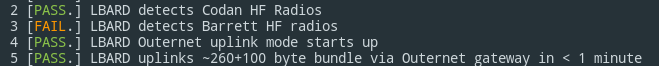
\includegraphics[width=14cm,height=20cm,keepaspectratio]{Figures/testOutput1.png}
        \caption{Example output of LBARD tests}
        \label{fig:exampleTest}
    \end{centering}
\end{figure}

The produced log file contains the outputs of all the programs run in the course of the test including \texttt{servald} and \texttt{lbard} instances, \texttt{fakeradio}, and the test framework, with each line in the log file timestamped.
The log files produced contain several pieces of information.
At the beginning of the file the name, status, and start/finish time of the test is listed.
Next, the complete logs of each of the started sub-processes are listed.
Tests can be configured to display more log information by setting specific flags in the configuration of the test.


\section{Limitations}
While the emulators are able to test large portions of the Serval network, they have several limitations that drastically limit the usefulness of the emulators to effectively model real world situations.
The first limitation is that it is currently not possible to model networks that use WiFi alongside radio, limiting the testable scenarios to that of just WiFi if using the Serval-DNA framework, or just radio networks if using the LBARD framework.

Another major limitation of the test frameworks is that there currently exists very few topologies that are being tested.
While the Serval DNA portion of the framework does feature various WiFi-exclusive topology tests including long node chains and a 6 node circular network these are minimal,
and the LBARD framework only features topologies of chain networks
Due to the previous limitation, this means there are no currently existing topology tests that contain multiple radio types or WiFi/radio networks.

While the log files produced by the tests are extensive and contain a large amount of data that is helpful while debugging, it does have several drawbacks.
Firstly, with just the log files and the status message it is difficult to determine where errors are occurring in a test, particularly in initial stages of debugging network topologies.
Partially, this is due to the log files not being chronologically ordered, but instead ordered by what log file it is, and \emph{then} chronologically ordered.
This means that attempting to work out where an error occurred becomes a process of consistently switching places in the large log file.
When more detail has been located about the issue — such as which device it occurred on, then it is useful to go through the large log file.

The log file has a further limitation, as the partially chronological ordered log has no information about network topology or graphical output, hindering efforts to explain network issues.

Finally, as topology tests have not been extensively tested, it is difficult to determine the simulation fidelity.
Without a comparison between the test framework and real-world scenarios, the simulation fidelity is impossible to determine. 
This can lead to a lack of confidence in the results of the emulated tests, and may lead to issues occurring in the real-world that do not occur in the emulation.


\section{Suggested Improvements}
To improve the LBARD test framework, multiple changes will need to be made.
The first of these is adding the ability to allows nodes to communicate over both WiFi and Fakeradio.
This step alone will drastically increase the scope of possible tests that can be conducted, as it will allow for tests of both WiFi and emulated Fakeradio interface.
Further, this will allow for networks to utilise more than one type of radio communication.

With the ability to have multiple link types between Serval nodes, a much larger range of network topologies can be modelled and tested.
Adding more network topologies to the test framework will allow for a much more detailed testing, and will almost certainly uncover previously undiscovered issues with the Serval network as it has simply not been possible to test complicated network topologies in emulation before.

To allow testers to more effectively debug the results of a test, a simpler log file will need to be generated.
This log file should contain only the crucial log information from a test, and the log lines should be formatted in a consistent format and chronologically ordered.

To improve on the ability to understand and communicate the functionality of specific Serval network topologies, some form of graphical output will need to be created, allowing for testers to see the network undergoing testing, as well as the data moving around the network.
This will almost certainly prove beneficial to the Serval team on two fronts. 
Firstly, this will assist Serval developers in isolating and locating bugs in Serval networks by visually showing them the functioning of a network, supplementing the expansive log files that the frameworks produce.
Further, this will assist Serval team members communicating where issues are occurring as the diagrams can act as a supplement to the explanation.

Finally, once the emulator can model a variety of network topologies, the simulation fidelity of the emulator should be determined.
To achieve this, the emulator should model a real-world Serval network and run tests on this network, and then those same tests should be run on a real-world implementation of this network.
This will serve to validate the accuracy of the Serval emulator, as it is expected that modelling the same network should have near-identical results with minimal variance provided the appropriate variables (i.e. average packet loss) have been accounted for in the emulation.

\section{Summary}
In this chapter we have answered the first research question "\firstRQ" as well as the third research question "\thirdRQ".
To analyse the state of the test framework, its aims first needed to be analysed. 
This aim of the Serval-DNA framework was determined to be: provide the basis for validating the functionality of core Serval functionality.
The aim for the LBARD framework was determined to be: provide the basis for field tests, and validate LBARD functionality, particularly the tree-synchronisation and the radio drivers.

In this chapter, both the Serval-DNA and LBARD test framework were analysed in detail, and an explanation and outline provided of their core functionality.
The process for defining tests and a detailed analysis of the two main output types of the frameworks was conducted.
The limitations of the frameworks was outlined, and then a list of recommendations of improvements that should be made to the test frameworks was listed, answering the third research question.
In the next chapter, the first of these improvements will start to be implemented, beginning the answering of the fourth research question "\fourthRQ.
The improvements that will be implemented is adding the functionality to allow WiFi to run alongside radio in a test and then more topology-focused tests will be added to the framework.